\chapter{Nachbildung des Quadrocopterfluges in Russland}
\label{chap:nachbildung_des_quadrocopter}
Mithilfe des Videos \cite{Anderson.2018} und den in der Beschreibung gemachten Angaben, soll der Flug eines Quadrocopters auf \SI{10,2}{km} Höhe im erstellten Tool nachgebildet werden. Es soll dabei die Validität des Modells und die Glaubwürdigkeit des Fluges an sich überprüft werden. 
\section{Komponenten des Quadrocopters}
\label{sec:komponenten} 
Im Folgenden sind alle technischen Daten, die im Programm eingebracht wurden aufgelistet. Diese sind aus dem Video und den Beschreibungen zu dem Quadrocopter entnommen worden. Fehlende Daten wurden geschätzt oder sind beim Piloten nachgefragt worden.
\subsubsection{Motor}
Der verwendete Motor war ein Cobra C2206/ 30 1400KV. Die technischen Spezifikation des Motors sind in Tab.\ref{tab:mot_cobra_parameter} aufgelistet. Es wurden kleine, sehr schnell drehende Brushless DC Motoren verwendet in Bezug auf den \ensuremath{K_V}-Wert und das Motorgewicht.
\begin{center}
	\captionof{table}{Motorparameter}
	\begin{tabular}{l l l} \hline
		 Parameter & Variablenname & Wert \\ \hline
		 Innenwiderstand \ensuremath{R_i} & \texttt{R\_i} & \SI{0,123}{\ohm} \\
		 Geschwindigkeitskonstante \ensuremath{K_v} & \texttt{K\_V} & \SI{1400}{RPM/V} \\
		 Leerlaufstrom \ensuremath{I_0} & \texttt{I\_O} & \SI{0,52}{A}  \\
		 maximaler Dauerstrom \ensuremath{I_{max}} & \texttt{I\_max} & \SI{40}{A} \\
		 Motormasse \ensuremath{m_{Mot}} & \texttt{m\_Mot} & \SI{0,0365}{kg} \\ \hline
	\end{tabular}	
	\label{tab:mot_cobra_parameter}
\end{center}

\subsubsection{Propeller}
Als Propeller wurden 4 Gemfan7038-Propeller eingesetzt. Das sind Propeller mit einem Durchmesser von \SI{7}{in} und einem Pitch von \SI{3,8}{in}. Für diesen Propeller wurde in der Leistungsberechnung ein äquivalenter Propeller aus der APC Datenbank mit den gleichen Abmessungen verwendet.

\subsubsection{Batterie}
Die Batterie ist eine selbst gebaute LiIon Batterie in der Bauform 4s3p. Das Gewicht einer Zelle beträgt ca. \SI{46}{g}. Mit dieser Angabe, kann das Gesamtgewicht der Batterie sehr gut abgeschätzt werden. Die nominale und die minimale Spannung pro Batteriezelle konnten aus den zusätzlichen Angaben berechnet werden. So betrug die Spannung der Batterie zu Beginn des Fluges ca. \SI{15,6}{V} und am Ende ca. \SI{11,5}{V}. Hierbei ergibt sich die nominale Spannung für eine 4-Zellen-Batterie zu \SI{3,9}{V} und eine minimale Spannung einer Zelle zu \SI{2.875}{V}. Alle weiteren notwendigen Spezifikationen sind in Tab.\ref{tab:bat_4s3p_parameter} festgehalten.
\begin{center}
	\captionof{table}{Batterieparameter}
	\begin{tabular}{l l l} \hline
		 Parameter & Variablenname & Wert \\ \hline
		 
		 Anzahl der Batteriezellen \ensuremath{N_{Bat,cell}} & \texttt{N\_bat\_cell} & \SI{4}{} \\
		 nominelle Kapazität einer Batteriezelle \ensuremath{C_{Bat,cell}} & \texttt{U\_Bat\_cell} & \SI{3120}{mAh} \\
		 nominale Spannung pro Batteriezelle \ensuremath{U_{Bat,cell}} & \texttt{U\_bat\_nom} & \SI{3,9}{V} \\
		 minimale Spannung pro Batteriezelle \ensuremath{U_{Bat,cell,min}} & \texttt{U\_bat\_min} & \SI{2,875}{V} \\
		 Peukert-Konstante \ensuremath{P}& \texttt{P\_bat\_Peukert} & \ensuremath{1,05} \\
		 Maximale C-Rate \ensuremath{C_{rate,max}} & \texttt{C\_Rate\_max} & \SI{30}{} \\
		 Batteriemasse \ensuremath{m_{Bat}} & \texttt{m\_bat} & \SI{0,55}{kg} \\ \hline
	\end{tabular}	
	\label{tab:bat_4s3p_parameter}
\end{center}

\subsubsection{Qudrocopterabmaße}
Die Maße des Rahmens und somit auch die Gesamtmaße konnten nur mit Bildern abgeschätzt werden. An dieser Stelle sind die vier Arme des Quadrocopters auf \SI{12}{cm} x \SI{2}{cm} und der Rumpf auf \SI{15}{cm} x \SI{5}{cm} angenähert worden.

\subsection{Missions und Umgebungsparameter}
Weitere Startbedingungen und Missionsparameter sind in Tab.\ref{tab:umgebungs_missions_parameter} dargelegt. In dem Video ist deutlich zu erkennen, dass die Steiggeschwindigkeit über der Höhe nicht konstant bleibt sondern zwischen \SI{15}{m/s} und \SI{0}{m/s} schwankt. Der Luftdruck und die Dichte am Abflugtag sind unbekannt und werden hier entsprechend der Standardatmosphäre angenommen.
\begin{center}
	\captionof{table}{Umgebungs- und Missionsparameter}
	\begin{tabular}{l l l} \hline
		 Parameter & Variablenname & Wert \\ \hline
		 Steiggeschwindigkeit \ensuremath{V_{Kg}} & \texttt{V\_Kg} & \SI{10}{m/s} \\
		 Erdbeschleunigung \ensuremath{g} & \texttt{g} & \SI{9,81}{m/s^2} \\
		 Starthöhe \ensuremath{H_0} & \texttt{H\_0} & \SI{0}{m} \\
		 Schrittweite der Höhe  \ensuremath{\Delta H} & \texttt{Delta\_H} & \SI{50}{m} \\
		 maximale Höhe \ensuremath{H_{max}} & \texttt{H\_max} & \SI{20000}{m} \\
		 Umgebungstemperatur am Start \ensuremath{T_0} & \texttt{T\_0} & \SI{263,15}{K} bzw. \SI{-10}{^\circ}\\
		 Luftdruck am Start \ensuremath{p_0} & \texttt{p\_0} & \SI{101325}{Pa} \\
		 Dichte am Start \ensuremath{\rho_0} & \texttt{rho\_0} & \SI{1,225}{kg/m^3} \\
		 Adiabatenexponent \ensuremath{\kappa} & \texttt{kappa} & \SI{1,4}{} \\
		 Windgeschwindigkeit \ensuremath{u_{Wg}} & \texttt{u\_Wg} & \SI{10}{m/s} \\ \hline
	\end{tabular}	
	\label{tab:umgebungs_missions_parameter}
\end{center}

\section{Nachbildung im Programm}
\label{sec:nachbildung_im_programm}

\section{Ergebnisse}
\label{sec:ergebnisse_quadrocopter}

\begin{itemize}
	\item \textcolor{red}{neue Bilder einfügen und Beschreibung entsprechend anpassen}
\end{itemize}





Im Nachfolgenden sind die Ergebnisse des Programms in Graphen dargestellt. Aus allen Diagrammen ist zu entnehmen, dass der Quadrocopter eine Höhe von mehr als \SI{13000}{m} erreichen kann. Das ist mehr als \SI{3000}{m} höher als die Höhe, die der Quadrocopter im Video erreicht.
Die Restladung der Batterie nimmt mit der Höhe linear ab (Vgl. Abb.\ref{pic:restladung_russland}).  
\begin{center}
	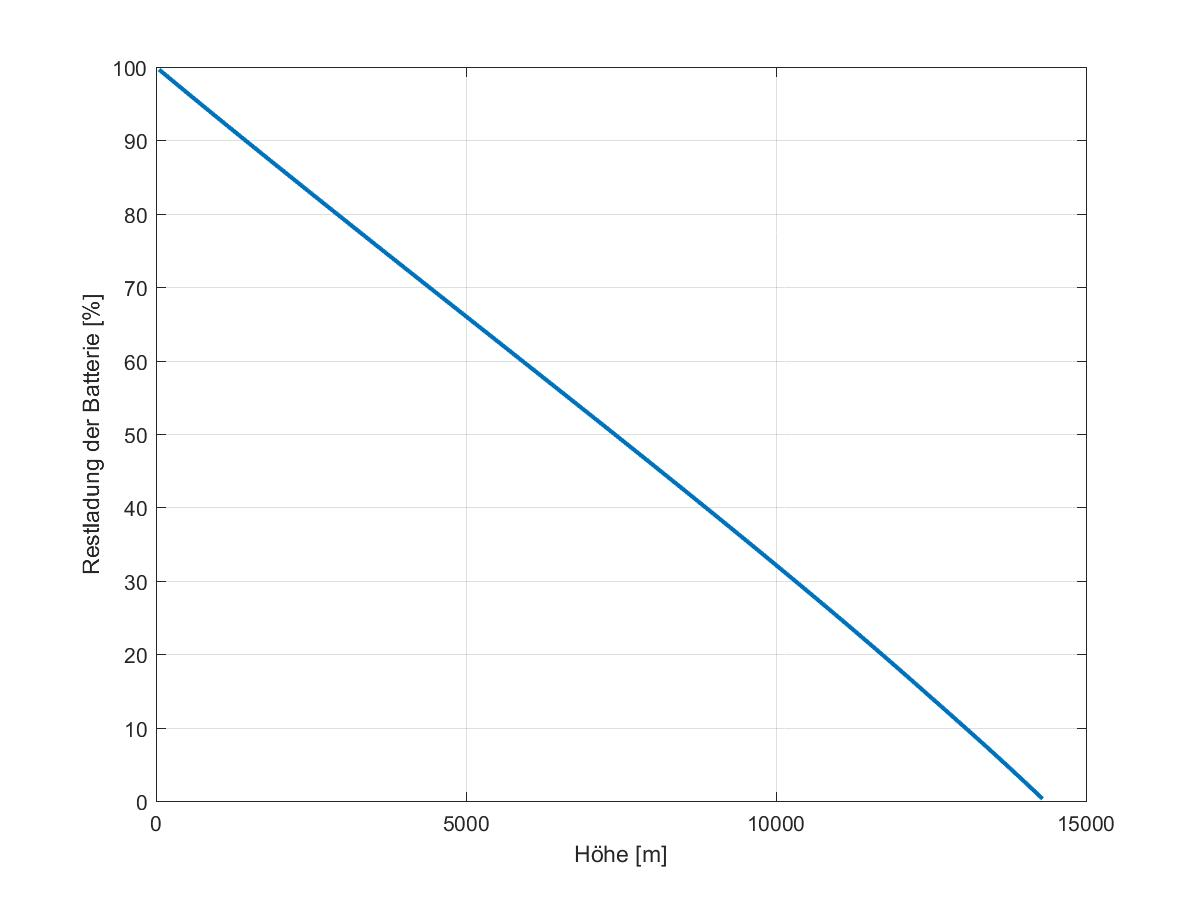
\includegraphics[scale=0.3]{Diagramme/C_Rest_V.jpg}
	\label{pic:restladung_russland}
	\captionof{figure}{Restladung der Batterie über der Höhe}
\end{center}
Diese erweist sich jedoch nicht als begrenzender Faktor, da selbst in \SI{13000}{m} Höhe immer noch ca. \SI{3}{\%} Restladung vorhanden sind. Im Video ist weiterhin die verbrauchte Kapazität in \SI{}{mAh} gegeben. Mit dieser und der Gesamtkapazität von aller Zellen kann daraus geschlossen werden, dass der Quadrocopter noch eine Restladung von etwas weniger als \SI{28}{\%} unter idealen Bedingungen am Top Of Climb (TOC) hat. Dieses stimmt beim Ablesen der Restkapazität in \SI{}{\%} bei \SI{10260}{m} aus dem Diagramm annähernd überein. Die berechnete liegt ziemlich genau bei der realen.
Hiergegen nimmt die Motordrehzahl und damit auch die Propellerdrehzahl leicht quadratisch zu und erreicht am TOC \SI{17000}{U/min} (Vgl. Abb.\ref{pic:omega_russland}).  
\begin{center}
	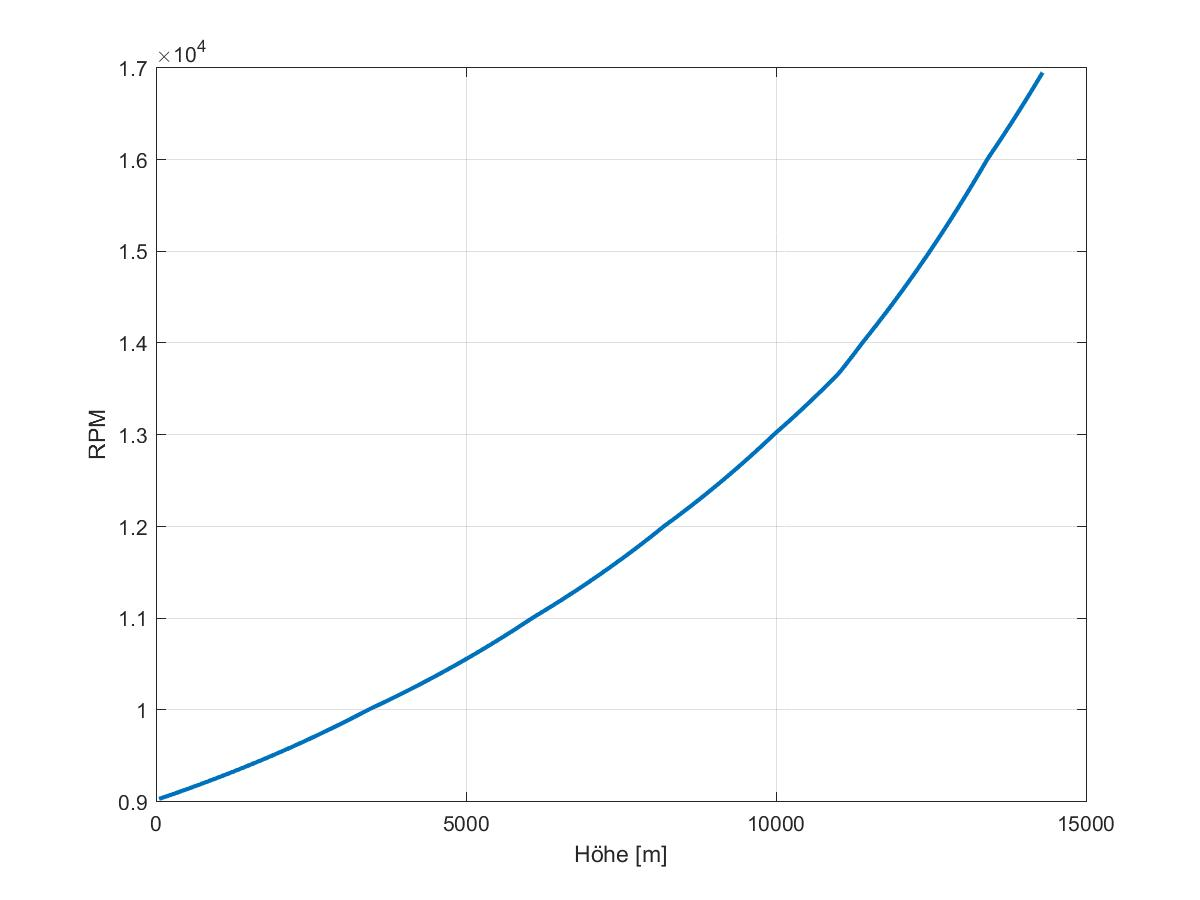
\includegraphics[scale=0.3]{Diagramme/omega.jpg}
	\label{pic:omega_russland}
	\captionof{figure}{Motordrehzahl der Batterie über der Höhe}
\end{center}
Dies entspricht auch der maximalen Drehzahl des APC-Kennfeldes. Die Berechnung wird abgebrochen, weil das Kennfeld für Drehzahlen von über \SI{17000}{U/min} keine Daten mehr liefert. Es ist daher zu vermuten, dass letztendlich die Restkapazität den limitierenden Faktor für größere Höhen  darstellt. Trotz der hohen Propellerdrehzahl erreicht die Blattspitzengeschwindigkeit \ensuremath{M_{tip}} mit \SI{0.6}{Ma} keine Ma = 1. Bemerkenswerterweise erreichen die Restladung und die Propeller-/Motordrehzahl simultan die vorher festgelegten Grenzen. \\
Der aus der Batterie entnommene Strom \ensuremath{I_Bat} bleibt innerhalb von \SI{22}{A} und \SI{25}{A} für den im Video erreichten Höhenbereich relativ konstant. 
\begin{center}
	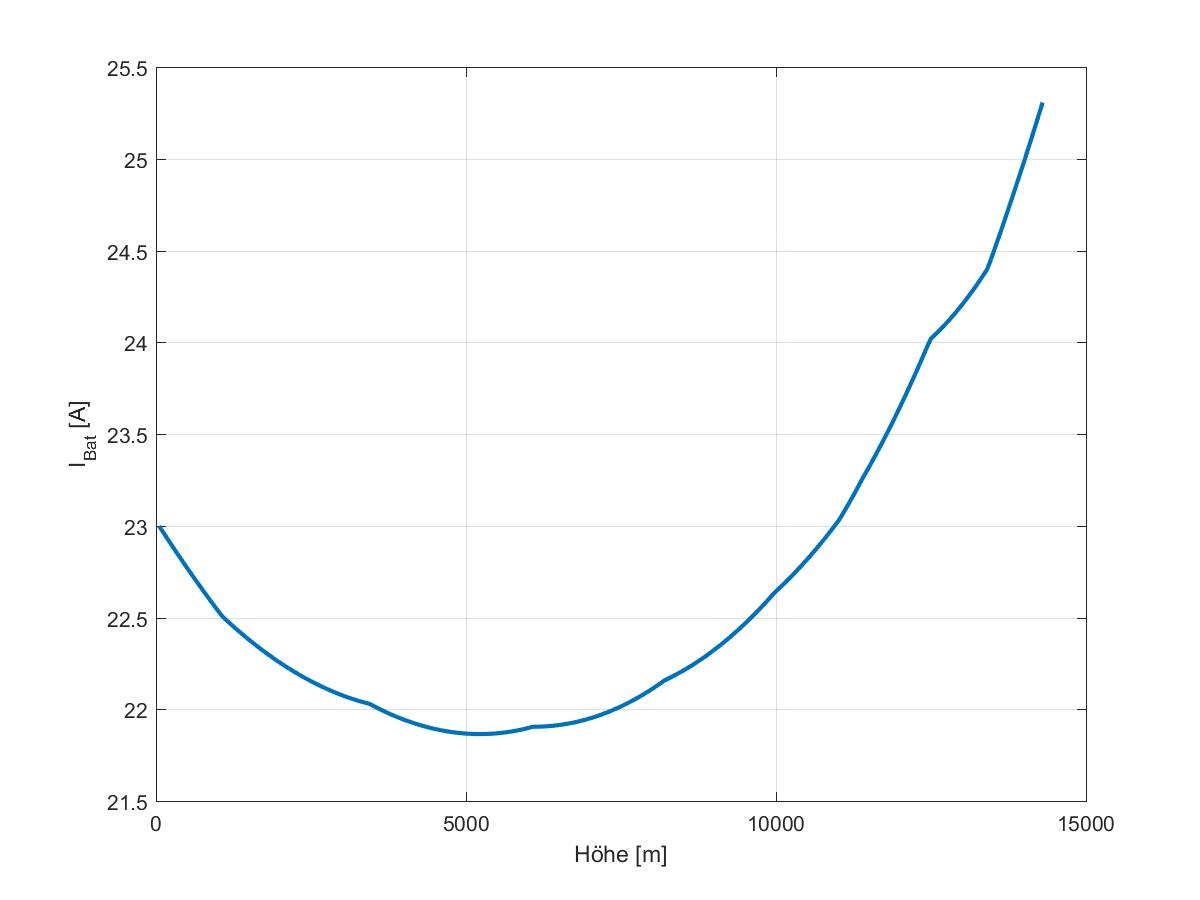
\includegraphics[scale=0.3]{Diagramme/I_Bat.jpg}
	\label{pic:batteriestrom_russland}
	\captionof{figure}{Entladestrom der Batterie über der Höhe}
\end{center}
Dies stimmt mit den Beobachtungen aus \cite{Anderson.2018} gut überein. In diesem schwankt der Entladestrom zwischen \SI{21,5}{A} und \SI{25}{A}.
Stimmen die oben genannten Größen mit denen im Video noch relativ gut überein, zeigen sich bei der PWM große Diskrepanzen. Die ermittelte PWM über der Höhe ist beim Start etwa \SI{50}{\%} und steigt im Laufe des Fluges auf ca. \SI{82,5}{\%} am TOC. 
\begin{center}
	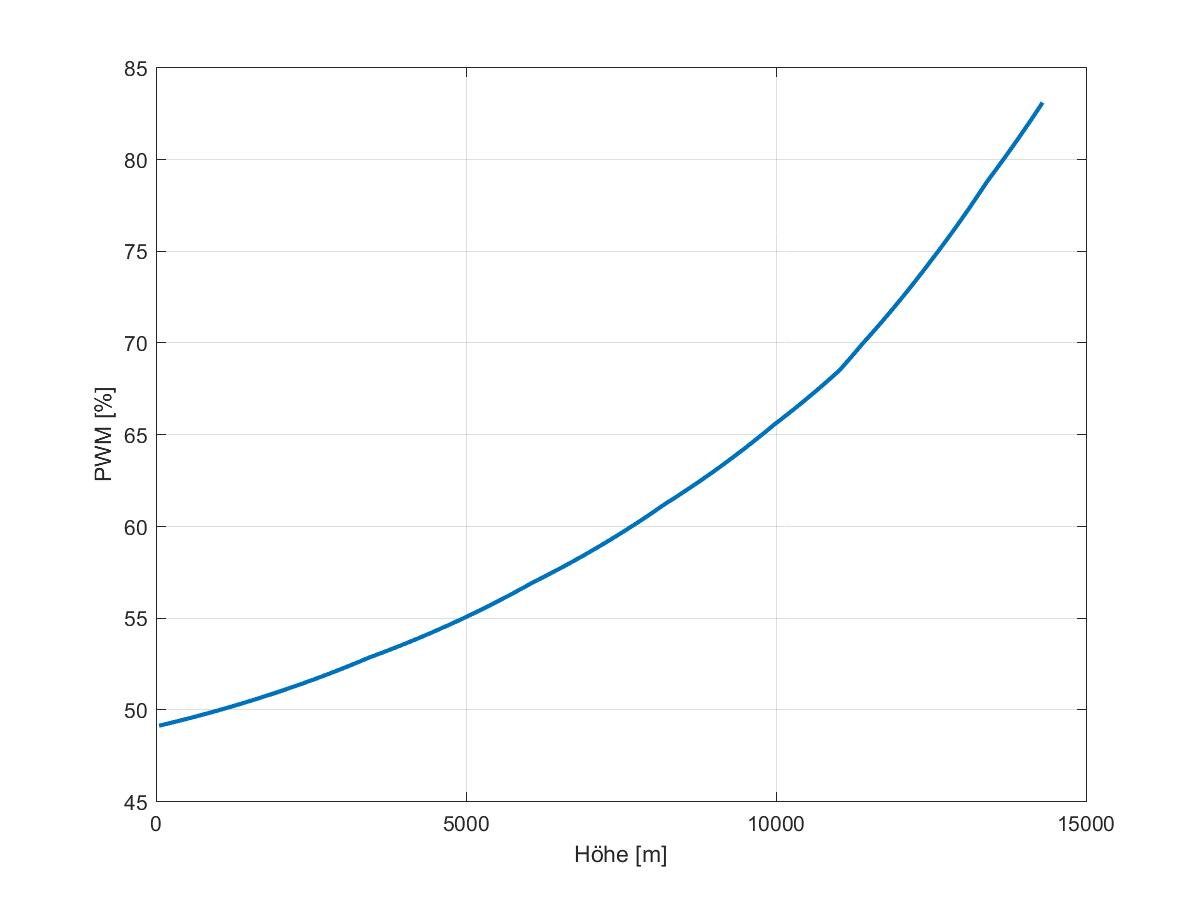
\includegraphics[scale=0.3]{Diagramme/PWM.jpg}
	\label{pic:pwm_russland}
	\captionof{figure}{Pulsweitenmodulation über der Höhe}
\end{center}
Der Vergleich mit dem realen Quadrocopterflug zeigt deutlich, dass die errechnete PWM im Durchschnitt etwa \SI{20}{\%} unterhalb der realen liegt.


\section{Diskussion}
\label{sec:nachbildung_diskussion}

Zusammengenommen wird der Quadrocopterflug in Russland sehr gut in dem Programm wiedergegeben. Die Flugghöhe ist um \SI{3000}{m} höher als die tatsächlich geflogene, jedoch wird in dem Programm die Batterie komplett entladen. Nichtsdestotrotz gibt es auch Abweichung.\\
Die verbleibende Kapazität im TOC im Programm wird mit Abweichungen von lediglich \ensuremath{\pm\SI{1}{\%}} exakt getroffen. Dies verwundert, da unter anderem der Stromverbrauch zusätzlicher Geräte wie der Motorregler, der Kamera, des Empfängers und anderer nicht in die Kalkulaiton mit einfließen. Außerdem werden dynamische Effekte (Vgl Kap.\ref{sec:vernachlaessigungen_vereinfachungen}) zum Ausgleich von Störungen verursacht durch Böen vernachlässigt. Diese sind in \cite{Anderson.2018} deutlich zu sehen. Als mögliche Ursache können die konservativen Berechnungsmodelle des Motors und des Motorreglers festgestellt werden. Generell wurden die Umgebungsbedingungen, was vor allem die Windgeschwindigkeit und die Atmosphäre betrifft, vereinfacht. Die Windgeschwindigkeit ist in der Nachbildung auf konstante \SI{10}{m/s} gesetzt worden. Auch wurde eine Standardatmosphäre vorausgesetzt wohingegen die reale Atmosphäre abweichen kann. Aus dem Video lässt sich jedoch entnehmen, dass relative Windstille am Flugtag herrschte und lediglich vereinzelte Böen in größeren Höhen in Erscheinung traten. Der Einfluss dieser kann trotzdem als gering eingestuft werden, gerade da die Standardatmosphäre und die konstante Windgeschwindigkeit eine gute Näherung liefern. \\
Weiterhin ist anzumerken, dass Koriakin mit deutlich abweichenden Steiggeschwindigkeit zu \SI{10}{m/s} aufgestiegen ist. In Programm wurde der Endzustand erreicht, wenn \SI{10}{m/s} nicht mehr fliegbar sind. Dabei werden geringere, eventuell noch fliegbare Geschwindigkeiten außer Acht gelassen. Eine kontinuierliche Verringerung der Geschwindigkeit auf \SI{0}{m/s} fand deshalb nicht statt. Unabhängig davon ist die Annahme einer Steiggeschwindigkeit von \SI{10}{m/s} akkurat. Der Steigflug mit dieser Steiggeschwindigkeit auf \SI{10260}{m} dauert \SI{17}{min} und \SI{6}{sec}. Dies ist gerade einmal \SI{11}{sec} kürzer als die tatsächliche Flugzeit von \SI{17}{min} und \SI{17}{sec} zum TOC in \cite{Anderson.2018}.\\
%Die signifikantesten Unterschiede zwischen Realität und Video sind bei der PWM gegeben, also dem Verhältnis zwischen Motorspannung und nomineller Batteriespannung. Die ermittelte PWM weicht im Schnitt um mehr als \SI{20}{\%} von der realen ab. Eine Ursache kann in dem Verhalten der Batteriespannung unter Last gefunden werden. In dem verwendeten Batteriemodell wird die nominelle Batteriespannung als konstant angesehen. Dieses berücksichtigt nicht den Spannungseinbruch unter Last oder die Spannung in Abhängigkeit des Entladezustandes. Diese Einflüsse beschreibt \cite{Tremblay.2009} in seinem Batteriemodell. Durch diesen Einfluss ist die tatsächliche Spannung geringer als die nominelle. Das könnte erklären, warum die PWM so bedeutend geringer ausfällt als in Wirklichkeit. \\ 
Die signifikantesten Unterschiede zwischen Realität und Video sind bei der PWM gegeben, also dem Verhältnis zwischen Motorspannung und nomineller Batteriespannung. Die ermittelte PWM weicht im Schnitt um mehr als \SI{15}{\%} von der realen ab. Selbst die Implementierung eines lastabhängigen Bateriespannungsmodells nach \cite{Tremblay.2009} brachte nur eine Verbesserung von lediglich \SI{5}{\%}. Eine Ursache kann in der Abriegelung des Motorstroms gefunden werden. Da zum Ausgleich von Störeinflüssen immer noch eine gewisser Leistungsüberschuss gegeben sein muss, wird die PWM ab einem gewissen Wert nach oben hin abgeriegelt. Dieses Verhalten wird in dem Modell nicht berücksichtigt. \\
Als weitere Einflüsse für die Abweichungen können die in Kap. \ref{sec:vernachlaessigungen_vereinfachungen} genannten Vernachlässigungen und Vereinfachungen aufgelistet werden. Ihr Einfluss auf die Gesamtabweichung kann allerdings als gering eingeschätzt werden.
% Weitere Einflüsse für die Abweichungen sollen an dieser Stelle noch aufgelistet werden. Ihr Einfluss auf die Gesamtabweichung kann allerdings als gering eingeschätzt werden. \\
%Unter anderem sind sehr einfache Modelle für die Motor, den ESC und die Batterie verwendet worden. Außerdem wurde ein Propeller von APC anstatt des originalen Herstellers verwendet. Durch den anderen Hersteller sind Unterschiede in Profilierung, Verwindung und Profiltiefenverteilung mit zu berücksichtigen. Abweichungen im Kennfeld beeinflussen die darauf aufbauende Berechnung. Dies wurde an dieser Stelle vernachlässigt.